\documentclass[titlepage,12pt]{report}

\usepackage[utf8]{inputenc}
\usepackage[a4paper, total={6in, 8in},headheight=14pt]{geometry}
\usepackage{newtxtext,newtxmath}
\usepackage[scaled=1]{couriers}
\usepackage[spanish]{babel}
\usepackage{microtype}
\usepackage[bottom]{footmisc}
\usepackage{fancyhdr}
\usepackage{graphicx}
\usepackage{blindtext}
\usepackage{scrextend}
\usepackage{tocloft}
\usepackage{parskip}
\usepackage{multicol}
\usepackage{subcaption}
\usepackage{wrapfig}
\usepackage{multicol}
\usepackage{verbatimbox}
\usepackage[nottoc, notlot, notlof]{tocbibind}
\usepackage{listingsutf8}
\usepackage{url}
\usepackage[square,numbers]{natbib}
\usepackage{adjustbox}
\usepackage[makeroom]{cancel}
\usepackage[hidelinks]{hyperref}
\usepackage[Glenn]{fncychap}
\usepackage{lastpage}
\usepackage{fancyhdr}

\bibliographystyle{unsrtnat}

\pagestyle{fancy}
\fancyhf{}
\fancyhead[R]{\rightmark}
\fancyfoot[C]{\leftmark}
\fancyfoot[R]{\thepage}
\renewcommand{\footrulewidth}{0.6pt}% Line at the footer visible
\addto\captionscatalan{%
  \renewcommand\contentsname{Índice}%
}

\fancypagestyle{plain}{%
  \fancyhf{}%
  \fancyfoot[R]{\thepage}%
  \renewcommand{\headrulewidth}{0pt}% Line at the header invisible
  \renewcommand{\footrulewidth}{0.6pt}% Line at the footer visible
}


\renewcommand{\cftpartleader}{\cftdotfill{\cftdotsep}}%
\renewcommand{\cftsecleader}{\cftdotfill{\cftdotsep}}%
\renewcommand\familydefault{\sfdefault}

\usepackage{tikz}
\usetikzlibrary{shapes.geometric, arrows}

\newcommand{\Lagr}{\mathcal{L}}
\newcommand{\Xagr}{\mathcal{X}}

\setlength{\skip\footins}{1cm}

\makeatletter
% \patchcmd{<cmd>}{<search>}{<replace>}{<success>}{<failure>}
\patchcmd{\@makechapterhead}{\huge}{\large}{}{}% for \chapter
\patchcmd{\@makechapterhead}{\Huge}{\large}{}{}% for \chapter
\patchcmd{\@makeschapterhead}{\Huge}{\large}{}{}% for \chapter*
\makeatother


\begin{document}

\iftrue
\newcommand{\HRule}{\rule{\linewidth}{0.5mm}}

\thispagestyle{empty}

\begin{center}

{\large Universitat Politècnica de Catalunya}

\medskip
{\large Facultat d'Informàtica de Barcelona (FIB)}

\vfill
{\bfseries\Large Bachelor's Degree Project}

\vfill
\centerline{\mbox{
\includegraphics[width=60mm]{media/FIB_UPC.png}}}

\vfill
\vspace{5mm}

{\LARGE Jordi Gil González}

\vspace{15mm}

% Title in English according to the official assignment
{\LARGE\bfseries Analysis of the Path Tracing \\ rendering method on CPU and GPU}

\normalfont \small \sffamily{}

\vfill

Computer Science Department


\vfill

\begin{tabular}{rl}
Bachelor's Degree Project Director: & Chica Calaf, Antoni \\
\noalign{\vspace{2mm}}
Study programme: & Computer Science\\
\noalign{\vspace{2mm}}
Specialization: & Computer Graphics\\
\end{tabular}

\vfill

\large Academic Year 2019/2020

\large \today

\end{center}

\newpage
\tableofcontents*
\fi

\newpage

\chapter{Contextualization and Scope of the project}

\section{Introduction} \label{introduction}

Nowadays, the images generated by computers are very present in both a work and entertainment environment. The creation of realistic images through computer programs has become a necessity. Industries like the film or video games need algorithms capable of representing the real world in a virtual one and, whenever possible, in the shortest possible time.

The study about methods that allow rendering realistic images is not new. Between the early and mid 70s, the first papers about the simulation of light and colours over the surface of three-dimensional models began to be published. To understand how these methods work, we have to keep in mind the common representation of 3D models.

To represent a 3D model it uses a ''polygon mesh'', commonly known as a triangle mesh because, the triangle, is the most used polygon. This mesh consists of a set of vertexes connected through edges and creating faces.  For all face, we can define an orthogonal normal vector. In Figure \ref{dolphin} we can see an example of a 3D model represented by a triangle mesh.

\begin{figure}[H]
	\centering
	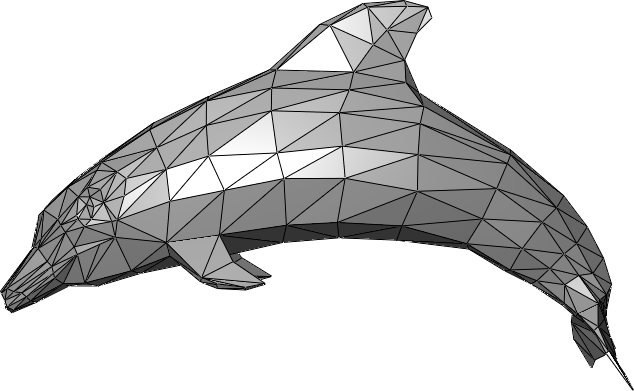
\includegraphics[scale=0.15]{media/Dolphin_triangle_mesh.png}
	\caption{Triangle mesh example. Source: Wikipedia}
	\label{dolphin}
\end{figure}

Returning to lighting calculation methods, the simplest is the \textit{Flat Shading}. This method only uses one of all the vertexes that make it up and her normal to determine the colour of each face of our mesh. In a mesh represented by triangles, it's commonly using the centroid of the triangle. The colour it's interpolated for each vertex. Every face is computed independently and this produces a visual difference result between continuous faces. In Figure \ref{flat:shading} we can see an object rendered using this method. We might think that adding more vertexes improve the results, but is not the solution because when more vertexes have our meshes, more memory is required and the problem would not be solved. If we zoomed in at the 3D model, we would see the same effect (known as Mach bands) \citep[pp.~5245--5250]{Lotto1999}.

\begin{figure}[H]
	\centering
	
\includegraphics[scale=0.5]{media/Flat-shading-sample.png}
	\caption{Example of \textit{Flat Shading}. Source: Wikipedia}
	\label{flat:shading}
\end{figure}

In the smooth shading methods, the colour change between pixels instead of faces. The result is a smooth transition of colour between adjacent faces.
In 1971 Henri Gouraud presents us in his paper \textit{Continuous Shading of Curved Surfaces} \citep[pp.~623--629]{Henri1971} the Gouraud Shading. With this method, we can add more continuity to the shading, unlike the Flat Shading. The great improvement concerning the method presented above is that it does not require a high-density mesh to simulate greater continuity. For each pixel it's intensity is determined by interpolation of the intensities defined at the vertex of each polygon.

\begin{itemize}
	\item For each vertex, a normal is defined as the average of the normals of the polygons to which said vertex belongs.
	\item Through the using of some lighting model,  e.g. the Phong reflection model, the intensity of each vertex is computed using the normal taken in the previous point.
	\item For each pixel, the intensity it's interpolated on every vertex to get his intensity.
\end{itemize} 

As we can see in Figure \ref{Gouraud:shading}, the results are notably higher, however, it does not represent the specular highlights. These would be a problem if they appear in the centre of a face.

\begin{figure}[ht]
	\centering
	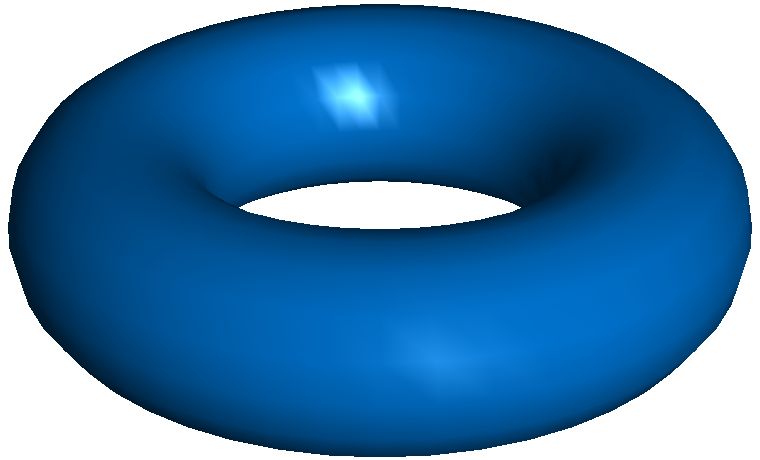
\includegraphics[scale=0.25]{media/Gouraudshading00.png}
	\caption{Ejemplo de \textit{Gouraud Shading}. Source: Wikipedia}
	\label{Gouraud:shading}
\end{figure}

Later, in 1975, Bui Tuong Phong in his PhD thesis \citep[pp.~311--317]{Phong1975} introduces to us the Phong Shading. In the method presented by Phong, instead of calculating the intensity at the vertex, first of all, the normal is defined, interpolated and normalized for each pixel and then using some lighting model the final intensity is determined. Computationally, this method is expensive regarding the others presented, because the calculation is made at fragment (pixel) level.

Phong mention in his paper published by the ACM \citep[p.~311]{Phong1975} that his goal was not to simulate the reality, but rather to add more realism:
\vspace{5mm}

\begin{mdframed}[hidealllines=true,backgroundcolor=gray!20] ''\textit{In trying to improve the quality of the synthetic images, we do not expect to be able to display the object exactly as it would appear in reality, with texture, overcast shadows, etc. We hope only to display an image that approximates the real object closely enough to provide a certain degree of realism.}'' 
\end{mdframed}

Even though these methods represented, as far as realism is concerned, an advance, they do not pretend to simulate reality. Furthermore, these only take into account ambient, diffuse and specular light. They do not take into account the indirect lighting of the scene, an important factor in creating images that produce realistic effects such as reflections.

It was not until the 80s that the first methods capable of rendering realistic images appeared. At the sixth annual conference on \textit{Computer graphics and interactive techniques (SIGGRAPH)}, Turner White presents the Ray Tracing method \citep[pp.~343--349]{Whitted1980}. This method is based on the Ray Casting algorithm, presented by \citep[pp.~37--45]{Appel1968}, consists of trace rays from the observer to all pixels, on for each one, to determine the closest object. Also, once the ray hits on a surface, based on the properties of the materials defined and the light properties, the colour is computed. In addition, using texture maps we can simulate shadows.

In 1986, David Immel et al. and James T. Kajiya, researchers from Cornell University and California Institute of Technology (Caltech) respectively, at the thirteenth annual conference on \textit{Computer graphics and interactive techniques (SIGGRAPH)} they introduced the \textit{Rendering Equation} \citep[pp.~143--150, pp.~133--142]{Kajiya1986, Immel1986}. This integral equation tries to summarize in one formula how the light interacts with a surface when a ray of light hits her using a bidirectional reflectance distribution function (BRDF). This formula takes into account the number of photons from the source, the incident angle, etcetera.

Exist other methods that can generate realistic images by approximating the RE: Bidirectional Path Tracing, presented by \citep[pp.~145--153]{Lafortune1993}; Photon Mapping, formulated by \citep[pp. ~21--30]{Jensen1996}; Metropolis light Transport, introduced by \citep[pp. ~65--76]{Veach1997}.

\newpage

\section{Contextualization}

\subsection{Context}

During the degree studies, there are several subjects dedicated to computer graphics. In these subjects, we are introduced to realistic rendering methods, but beyond the theoretical introduction to these, they are never put in practice. From here comes the idea of realizing the present project, to be able to go deeper into the subject of realistic rendering and thus create an application based on what has been learned during the studies. Other aspects of computer science seen will also put into practice, such as the creation of parallel applications on both CPUs and GPUs.

As we have pointed out in the last section, rendering true-to-life images is an area of great interests in computer graphics. One of the principal goals is to be able to render images that are indistinguishable from photographs. Following this idea, being able to replicate the behaviour of light in a virtual environment is an important task. It's essential to keep in mind the global illumination of our scene to achieve that realism. The global illumination is compounded by \begin{enumerate*}[label=\roman*)] \item direct illumination \label{item:dl} and \item indirect (global) illumination \label{item:il} \end{enumerate*}. In Figure \ref{globalil}, we can observe a graphic representation of both types of lighting.

\begin{figure}[!ht]
	\centering
	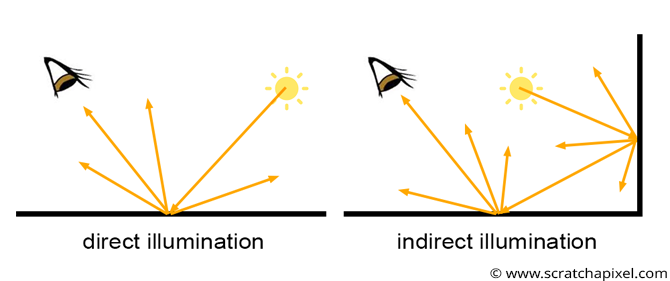
\includegraphics[scale=0.45]{media/shad2-globalillum3.png}
	\caption{Example of \textit{Direct illumination and Indirect illumination}. Source: ScratchPixel}
	\label{globalil}
\end{figure}

\ref{item:dl} Direct illumination is that which strikes a point from the light source.\\
\ref{item:il} Indirect illumination is that which hits one point from the light bouncing off other points in the scene.

Retrieving what was said in the introduction, the first method capable to render realistic images was the Ray Tracing, based on Ray Casting algorithm, a technique that consists in trace rays from the eye or camera to all pixels of an image. The great novelty concerning the algorithm presented by Appel is the recursivity. The Ray Tracing algorithm emits a ray from the virtual camera across the scene to a light source. When a ray hits some surface can produce three new types of rays: \begin{enumerate*}[label=\roman*)] \item
 reflection ray \label{ray:reflected}, \item
 refraction ray and \item
 shadow ray\end{enumerate*}. From this point, a new ray is projected until hits one of the light sources in the scene. When tracing new rays, we can obtain effects like reflections, shadows, caustics, etcetera. If the ray hits a transparent material like glass, the ray is projected through this to simulate the refraction rays. The principal disadvantage is the dependency on the number of polygons in the scene. The more polygons the scene will have, the more inefficient will be the algorithm.

The results obtained are not necessarily photo-realistic despite offering a high degree of realism by being able to accurately treat optical effects such as refraction or reflection. It's mandatory to do some post-processing to be able to simulate effects such as soft shadows or caustics. Rendering photo-realistic images is mandatory approximating the RE. The Path Tracing algorithm, presented by \citep[pp. ~143--150]{Kajiya1986}, is a good example of that.

The Path Tracing algorithm came up as an improvement of the Ray Tracing with the purpose to give a resolution of the rendering equation by the Monte Carlo integration. It is for this reason that the algorithm is inherently able to simulate effects such as motion blur, ambient occlusion and global illumination without any post-processing. Unlike Ray Tracing, in the Path Tracing when a ray is emitted by the virtual camera, this is traced through the scene bouncing in the objects until reaching one light source or sky or run out a limit. The significant difference between the algorithm presented by White is that the algorithm introduced by Kajiya, for each pixel, we keep in mind not only one ray but dozens, hundreds or even thousands. The random sampling is a significant aspect, this means that when a  ray hits a surface, it generates a new ray in a random direction. Once a ray reaches a limit or it is absorbed by a light source, the colour is computed according to the material properties of the objects it has bounced off. This colour is added to compute the average between all rays emitted for each pixel. This random sampling produces a noisy result. The more sampling we use, the smoother it becomes.

\begin{figure}[!ht]
	\centering
	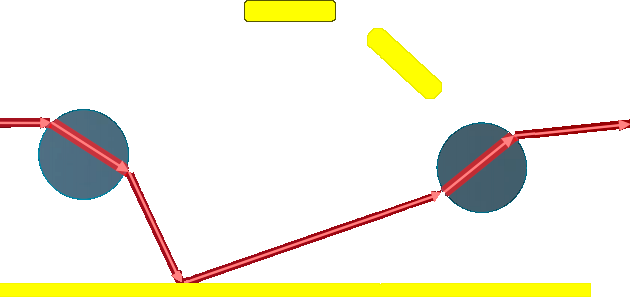
\includegraphics[scale=0.45]{media/lightPathRT.png}
	\caption{Ray Tracing}
	\label{RT_traced}
\end{figure}

\begin{figure}[!ht]
	\centering
	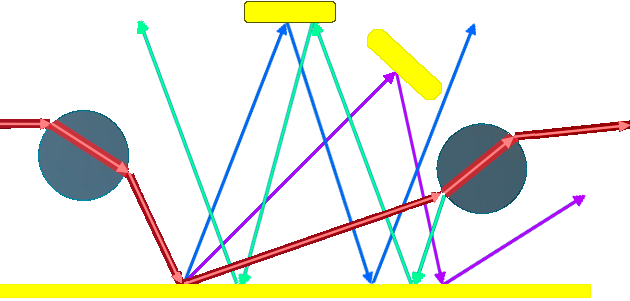
\includegraphics[scale=0.45]{media/lightPathPT.png}
	\caption{Path Tracing}
	\label{PT_traced}
\end{figure}

In Figure \ref{RT_traced} it can be observed what is mentioned in the previous paragraph. In the Ray Tracing, the colour calculation in one pixel depends only from the primary ray and his bounces until reach a light source. However, in Figure 5 it can be observed that for each bounced, multiple rays are traced. This occurs because when a ray hits a diffuse surface, the photons are scattered in all directions. 

The number of polygons in a scene is irrelevant for Path Tracing, the scene complexity does not affect proportionally the algorithm's performance. How we mentioned above, in the first method only one ray is traced for each polygon. However, in Kajiya's method, the ray is traced per pixel. Because each pixel is independent of each other, we can exploit the concurrency provided by CPUs and GPUs.

\begin{figure}[H]
	\centering
	\begin{subfigure}{.3\textwidth}
		\centering
		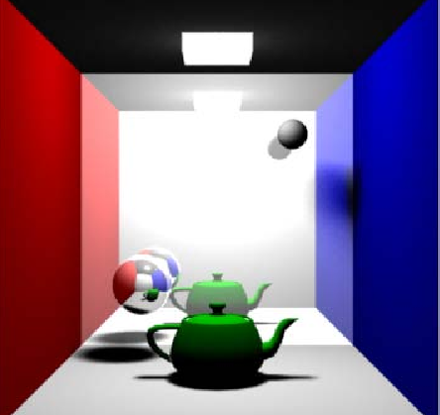
\includegraphics[width=.8\textwidth]{media/RayTracing.png}
		\caption{\textit{Ray Tracing}.}
		\label{RT}
	\end{subfigure}
	\begin{subfigure}{.3\textwidth}
		\centering
		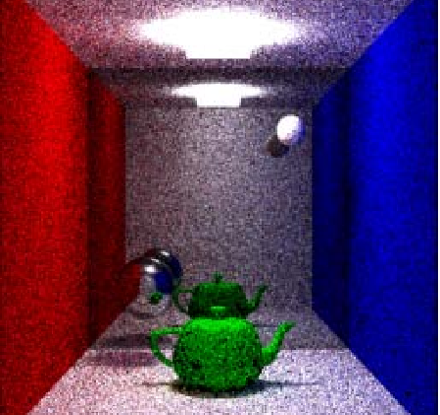
\includegraphics[width=.8\textwidth]{media/PathTracing.png}
		\caption{\textit{Path Tracing} with noise.}
		\label{PTN}
	\end{subfigure}
	\begin{subfigure}{.3\textwidth}
		\centering
		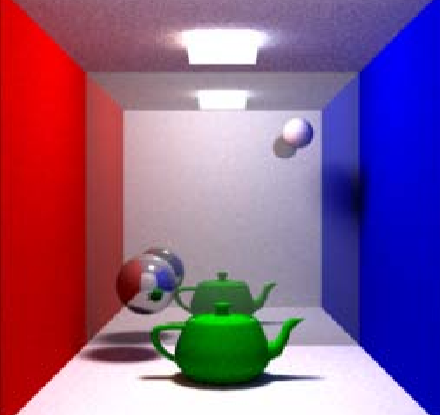
\includegraphics[width=.8\textwidth]{media/PathTracingMD.png}	
		\caption{\textit{Path Tracing} without noise.}
		\label{PT}
	\end{subfigure}
	\caption{Comparison \textit{Ray Tracing vs. Path Tracing}. Source: \citep[pp.~23--29]{Cassagnabere2004}}
\end{figure}

We can observe how the Path Tracing, in Figure \ref{RT}, produces soft shadows compared to Ray Tracing, Figure \ref{PT}. Also, we can see the noisy effect produced by the random sampling of Path Tracing if the number of samples is poor.

In that present project, we are going to create an application that implements the Path Tracing method trying to generate images that looks realistic. This application it's going to compute each pixel of an image given some scene. There will be three versions. The first one is the sequential version, where one pixel is computed at once and it's the base for all other versions. The other two versions are the CPU and GPU parallel versions. The reason to develop all of these versions is to be able to do a performance analysis about our algorithm both in GPU and CPU and decide which architecture is bringing more performance.

The implementation proposed by Peter Shirley in his books about Ray Tracing  \citep{ShirleyRTA, ShirleyRTB, ShirleyRTC} is going to be the base to develop our Path Tracer. The main intention is to develop three applications (sequential in CPU, parallel in CPU and GPU) to analyze how is the performance in both architectures CPU and GPU.

We will not only focus on the rendering section, although this is the central thread of this project, but we will also study which acceleration techniques are commonly used to try to improve our algorithm as much as possible. That is why we will also study which is the best way to represent internally the scene we want to render following the idea presented by \citep{Karras2012} in his paper.

The way we represent our scene will have a great impact on how we compute the colour of the final image. As we have mentioned above, the basis of the method is to trace rays through the scene to compute the colour of each pixel. If our representation of the scene consists of storing all the objects in a data structure such as a list or vector, ordered by order of creation, when calculating a point of the image in the worst case we will be going through the whole set of polygons of the scene to determine the final colour. Trying to render a scene that, very possibly, is composed of millions of polygons can translate into hours and hours of processing. That's why we'll make use of an accelerating data structure that allows us to represent the scene in a more clever way, so that when determining if a ray hits or not a polygon is determined in the fastest way possible.

\subsection{Stakeholders}

In this section, we are going to describe the different actors involved in a project.

\subsubsection{Developer}

This actor is in charge of planning, information search, documentation, development of the necessary software, solution of possible obstacles and problems that may arise throughout the development, and performance and analysis of the experiments. He needs to work in coordination with the director, and co-director if it exists and is the last person in charge of fulfilling the established terms.

\subsubsection{Project director}

This actor is in charge of leading the developer in case of difficulties, as well as advising on possible solutions.

\subsubsection{Benefited users}

Despite this project has not the intention to create a product on its own, it doesn't mean that there are not benefited users. Investigating the different ways of optimization using parallel architectures can be useful for many researchers or developers.

\section{Justification}

As we have already pointed in the above section, we will start from the Peter Sherly books and Tero Karras paper about Bounding Volume Hierarchies. In this project, we expect to study how we can exploit at maximum the different architectures that we have in our computers (CPU and GPU) and decide how's more efficient. We cannot compare our application with an existing one. Because the professional applications that implement the Path Tracing algorithm are made by experts with plenty of experience and knowledge that will allow increasing the performance significantly, and the author of this project does not have. Moreover, in the field of realism, it's hard to compare because a professional application includes plenty of features such as subsurface scattering or tessellation. In this project, it's impossible to reach an application with similar characteristics. First of all, the lack of knowledge and experience in the field of realistic off-line rendering.
Finally, the time. Usually, a project with this scope involves plenty of specialists and need months or years to realise. A professional example of Path Tracer is RenderMan, developed by Pixar Animation Studios \citep{Christensen2018}.

For this reason, in this project, we will develop three versions of the same algorithm: \begin{enumerate*}[label=\roman*)] \item sequential version, \item parallel version in CPU and \item parallel version in GPU \end{enumerate*}. Therefore, we will analyze the versions with each other and decide the best architecture and version for our implementation.

Currently, there are plenty of libraries oriented to GPU programming. Libraries such as \texttt{OpenCL} and \texttt{OpenACC} provides us with portability between graphics cards from different manufacturers like \texttt{AMD} and \texttt{NVIDIA}. For this project, we decided to choose the CUDA environment developed by \texttt{NVIDIA}. \texttt{CUDA} is a parallel computing platform and API created for its graphics card and accelerators. The reason we chose this API is that being proprietary software it is more optimized for \texttt{NVIDIA} graphics cards, as indicated by \citep{Karimi2010} and \citep[pp.~216--215]{Fang2011} in their respective papers.

It is possible that citing the \texttt{NVIDIA} graphics cards and accelerators and, keeping in mind the project's focus on rendering realistic graphics, to the lector of this Final Degree Project comes to mind the new brand of RTX cards designed by \texttt{NVIDIA}. In the beginning, the idea was to orient the project to use RTX graphics cards because they have been designed specifically for the use of Ray Tracing in real-time. But, this idea was immediately rejected because of the high price of these. The price range varies between 350€ to 2000€ or 6000€ (for HPC). Finally, even the author of this project bought an RTX 2080 Super it was decided not to focus the project only in the new RTX technology. Exploring all the new features that these include such as RT Cores, Tensor Cores and Mesh Shaders would have meant starting the job all over again and losing a huge amount of time spent. Because it would have been necessary to learn all the necessary knowledge to develop the project. That does not imply that the graphics card should not be used. As a high-end graphics card, the number of cores it has compared to the GTX1050 (mid-range) will allow us to analyse how much better it is and whether or not it is worthwhile, in terms of cost/power ratio, to use it in applications of this type.

As we mentioned at the beginning of this section,  \texttt{CUDA} is an API very optimized for \texttt{NVIDIA} hardware. This gives us an advantage because all the environments that we will use in this project have NVIDIA technology

\begin{enumerate}
	\item Laptop - Lenovo Legion Y520 with an Nvidia GTX1050 Mobile - 4GB.
	\item Personal Computer - Nvidia RTX 2080 Super - 8Gb.
	\item Teaching cluster BOADA - 4 GPUs Nvidia Tesla K40c.
\end{enumerate}

The use of graphics cards in different environments will allow us to analyse how our application responds in each of them and thus study how performance is when we use several cards designed for a research/professional environment, as opposed to two others designed for more ordinary use. We will also be able to see how the performance is in a mid-range graphics card (Nvidia GTX1050 Mobile) and a high range one (Nvidia RTX 2080 Super) and make a comparison between them.

\section{Project Scope}

To solve the problem presented in our project, we need an application that can render realistic-look images. As well we notice a few sections back, \citep{ShirleyRTA, ShirleyRTB, ShirleyRTC} presents the principles to create a Ray Tracing. We are going to use this to develop our main parallel application on CPU and GPU.

Furthermore, as we said in the context section, the use of acceleration structures is a significant factor in this type of applications, and they have been studying for many years by the science community, e. g.\citep{Rubin1980}. In this project, we will use the \textit{
Bounding Volume Hierarchy} (BVH), a tree structure (binary or n-ary) where each leaf represents the bounding box of each primitive; and each internal node the bounding box of his children.

There are many ways to build a BVH, but we decided to develop the version proposed by \citep{Karras2012, Karras2013}. We can build each internal node independently using the concurrence provided by the GPU and CPU.

\subsection{Objectives}

\subsubsection{Main objectives}

There are several main objectives that we propose in the project. The first one is to develop three applications (sequential, CPU parallel and GPU parallel) in which given a scene will render it using the \textit{Path Tracing} method, and we will analyze the performance given by all versions developed to determine who have a better performance.

A second main objective is studying and implementing what are the best practices about memory management in a parallel application. We identified it as one of the main goals because inadequate management of it can be a serious obstacle in the development of the project.

\subsubsection{Secondary objectives}

The secondary objectives, but no less important, are the following:

\begin{enumerate}
	\item Efficiently implement the methods presented by Peter Shirley and Tero Karras.
	\item Find information about optimization techniques in the calculation of ray-object intersection.
	\item Efficiently implement ray-object intersection calculations.
	\item \label{3D} Extend the application to render 3D models.
	\item \label{GLUT} Develop an interactive application.
\end{enumerate}

The secondary objectives \ref{3D} and \ref{GLUT} will be realised according to the time remaining for the completion of the project.

\subsection{Obstacles and risk}

Although the main topics dealt with in this project have been thoroughly studied, this does not mean that the development of this project is an easy task since there are many problems or obstacles that we may face.

\subsubsection{Main program}

As we said in the previous section, the memory management it's very important. An improper manage of this may cause errors that don't allow the correct functioning of the application.

\subsubsection{Algorithm}

The algorithm that we will use computes the colour from the ray-object intersection. In the process of generating an image, these intersections are made billions of time, so an improper/inefficient implementation of the calculations can affect the performance of our application negatively.

\section{Methodology and rigour}

In this section, we're going to look at the set of tools that we're going to use during the development of the project. To be able to carry out a good development of the project, we will organize ourselves in the following form: \begin{enumerate*}[label=\roman*)] \item Meetings every 15 days with the director to discuss the state of the project, results obtained, objectives fulfilled and determine the next steps. \item Meetings weeklies in the final phase. \end{enumerate*}

\subsection{Methodology}

The work methodology that we will follow in this project is agile. This methodology breaks development in small task to minimize the amount of planning. Each iteration, or sprint, has a set of assignments. In our project, each iteration of the development cycle will correspond with a meeting with the director until the next meeting. All meeting needs specifying the objectives to achieve to the next sprint. In Figure \ref{agile}, we can see a scheme of how agile methodology works.

\begin{figure}[ht]
	\centering
	
\includegraphics[scale=0.25]{media/agile.png}
	\caption{Agile methodology scheme. Source: OpenWebinars}
	\label{agile}
\end{figure}

\section{Development tools}

The programming language that we will use to develop our project is English using the \texttt{OpenMP} and \texttt{CUDA} libraries.

\texttt{OpenMP} is an API design to add concurrence to programs written in \texttt{C}, \texttt{C++} and \texttt{Fortran}. The main advantage against others with similar characteristics is the portability between different Operating Systems.

\texttt{CUDA} is a parallel computing platform and \texttt{API} developed by \texttt{NVIDIA} that allows us access to a set of instructions and compute elements inside the graphics cards and accelerators to create parallel applications.

\section{Monitoring tools}

To monitor the development of this project, we will use git to track all versions and consult them if necessary.

\chapter{Project Management}

\section{Planning}

This chapter deals with project planning and describes the tasks performed, through an action plan, to meet the deadlines relating to the delivery of the project. We will also present the resources used and analyze the possible obstacles that could modify the planning.

The project began in early July 2019 with a deadline on 13 January 2020. Finally, the delivery was postponed to April of the same year.

\section{Task description and resources used}

\subsection{Task description}

\subsubsection{Study of concepts}

Before starting the project, it was necessary to become familiar with the basic concepts relative to our project. There were a couple of meetings with the project director, during the previous semester, to define the topic of the project. Also, the author of this project enrolled in the subject of Graphics Cards and Accelerators (TGA for her acronym in Catalan) to introduce himself in the parallel computing platform \texttt{CUDA}. Since this task is carried out outside the project plus the difficulty of determining an estimate in hours, it will not be taken into account in the planning.

\subsubsection{System configuration}

Before starting the development, we need to configure the necessary tools and guarantee her correct functioning.

To be able to develop our project it is mandatory to have installed \texttt{CUDA} in our systems. The \texttt{OpenMP} libraries are installed by default on Linux systems, so no installation is required, but it is necessary to check that they work properly. To finish, we will make use of \textit{TexMaker}, a word processor that allows to us compile \LaTeX code to create our documentation.

The laptop and personal computer need setting up. The BOADA Cluster no needs a previous configuration because it has already been configured by the DAC (Departament d'Arquitectura de Computadors).

\subsubsection{Project Planning}

This task corresponds to the content covered by the GEP course. We can split them into three sub-tasks:

\begin{enumerate}
		\item Context and scope of the project.
		\item Time planning.
		\item Budget and sustainability.
\end{enumerate}

\subsubsection{Development}

Development task is the most important of all project. Includes the development of all three applications, results and documentation. We will split this phase in cycles of 14 days each one. Each cycle will have four subtasks:

\begin{itemize}

	\item \textbf{Sequential version development:} This version is the basis for the parallel applications.
	
	\item \textbf{CPU parallel version development:} Once the sequential version has been developed, we will translate them to CPU parallel version using the \texttt{OpenMP} library. 
	
	\item \textbf{GPU parallel version development:} Once the sequential version has been developed, we will translate them to CPU parallel version using the \texttt{CUDA} library. 

	\item \textbf{Results:} Using the three applications, we will render the defined scenes and will study the performance in each one of them.

\end{itemize}

The dependencies between the different tasks are easy to explain. Until we have not the sequential version, we can't start programming the parallel versions of this one. Nor can we start a new cycle without having finished the previous one.

\subsubsection{Final stage}

In this stage, we will structure all the documentation of the previous stages and prepare the defence.

\subsection{Summary table and estimation}

\begin{table}[H]
	\centering
	\begin{tabular}{|m{5cm}||m{5cm}|}
		\hline
		Task & Time spent (horas) \\ \hline \hline
		System configuration & 10 \\ \hline
		Project planning & 133 \\ \hline
		Development & 546 \\ \hline
		Final Stage & 65 \\ \hline \hline
		Total & 754 \\ \hline
	\end{tabular}
	\caption{Hours Summary}
\end{table}

With an estimation of 35 hours per week (3 hours from Monday to Thursday and 10 hours Saturdays and Sundays), and keeping in mind a total of 30 weeks of work, we have $35h*30 = 1050$ hours estimated.

\subsection{Resources used}

\subsubsection{Software}

\begin{itemize}
	\item Linux, used in all task.
	\item \LaTeX , for documentation.
	\item \texttt{C++},\texttt{OpenMP} and \texttt{CUDA}, for the development of the applications.
	\item \texttt{git}, used for version control and code sharing between different environments.
\end{itemize}

\subsubsection{Hardware}

\begin{itemize}
	\item Desktop PC with the following features: i7 7700 3.6 GHz, NVIDIA GeForce RTX 2080 SUPER, 24GB RAM, 250 SSD, 1TB SSD, 1TB HDD
	\item Laptop with the following features: i7 7700HQ 2.8GHz, NVIDIA GeForce 1050 Mobile, 8GB RAM, 500GB SSD
	\item Teaching cluster with the following features: Intel Xeon E5-2620 v2 2.10GHz x2, NVIDIA Tesla K40c x4, 64GB RAM, 1TB x2
\end{itemize}

\section{Risk management: Alternative plans and obstacles}

During the development may occur some obstacles or deviations that can alter the initial planning. Thanks to the agile methodology, it is easy to manage the mishaps that may arise. The main objectives were clearly and concisely defined, and this has allowed us to know in all moments which goals have been reached and have not.

The hours planned for the different task are not static. We may need more hours, or we may even have hours left over that we can spend on other tasks.

Besides, in the case of not being able to provide different shapes to represent our 3D models such as spheres or triangles, we will only use triangles because of the versatility that these give us.

\section{Knowledge Integration}

Principally, the knowledge integrated into the project corresponds to the knowledge acquired in the Computer Science speciality, as well as some obligatory subjects of the degree and optional ones. The familiarity about realistic rendering and application of geometric transforms on 3D objects, discussed in the subject of graphics, has been required. Also, the topics studied in subjects such as Parallelism and TGA, have been very important to develop our parallel applications.

Having knowledge in programming in languages like \texttt{C} or \texttt{C++} has been important for the proper development of the project.

\section{Identification of laws and regulations}

As we said in the first delivery, the main objective of the project is to allow the author to enter the field of computer rendering, in particular realistic rendering. For this reason, there are no laws or regulations that can be applied because it is not intended to make a commercial product. Furthermore, all the materials and tools used during the project are for free use or self-created.

\chapter{Budget and sustainability}

In this chapter, we will present two significant topics, budget and sustainability. We will provide a detailed description of the costs of the project, of both material and human resources, and an analysis of how the different obstacles that may occur during the development could change our budget. We will also assess the sustainability of the project.

\section{Budget}

In this section we will make an estimate of the budget to develop the project. We can divide the budget in two big sections: \begin{enumerate*}[label=\roman*)] \item Direct costs and \item Indirect costs \end{enumerate*}.

\subsection{Direct costs}

We divide the direct cost into the three types of resources that we have in the project: \begin{enumerate*}[label=\roman*)] \item software \item hardware and \item human \end{enumerate*}.

For the calculation of the amortization, we will take into consideration that the project has a duration of approximately eight months.

\subsubsection{Software resources}

All the software that we will use in our project is open source. The table \ref{soft} shows the cost of all software used.

\begin{table}[H]
	\centering
	\begin{tabular}{|c|c|c|c|}
		\hline
		\textbf{Product} & \textbf{Price} & \textbf{Lifetime} & \textbf{Amortization} \\ \hline \hline
		Ubuntu 18.04 	& 0,00€ & - & 0,00€ \\ \hline
		\LaTeX\ 		& 0,00€ & - & 0,00€ \\ \hline
		CUDA 			& 0,00€ & - & 0,00€ \\ \hline
		OpenMP 			& 0,00€ & - & 0,00€ \\ \hline
		C++ 			& 0,00€ & - & 0,00€ \\ \hline	\hline
		Total 			& 0,00€ & - & 0,00€ \\ \hline
	\end{tabular}
	\caption{Software resources cost}
	\label{soft}
\end{table}

\subsubsection{Hardware resources}

The table \ref{hard} shows the cost of all hardware used to develop the project. The amortization takes into account an approximate duration of eight months of the project as we have specified at the beginning of this section. Approximately one year have 365 days and the lifetime of the machines used is 5 years, then this gives us a total of 1825 days of life for the computers. The project lasts from September to April therefore the total duration is 243 days.

\begin{table}[H]
	\centering
	\resizebox{\textwidth}{!}{\begin{tabular}{|c|c|c|c|c|}
		\hline
		\textbf{Product} 	& \textbf{Price} & \textbf{Lifetime (in years)} & \textbf{Amortization/day} & \textbf{Amortization} \\ \hline \hline
		Desktop PC 		& 2210,09€ & 5 & 1,21€/día & 294,03€\\ \hline
		Lenovo Legion Y520 	&  900,00€ & 5 & 0,49€/día & 119,07€ \\ \hline
		BOADA 				& 3500.00€ & 5 & 1,92€/día & 466,56€ \\ \hline \hline	
		Total 				& 6610.09€ & - & -         & 879,65€ \\ \hline
	\end{tabular}}
	\caption{Hardware resources cost}
	\label{hard}
\end{table}

In the cost of the teaching cluster, BOADA, the four \texttt{NVIDIA Tesla K40c} graphics cards are not taken into account because they were a donation from \texttt{NVIDIA}, so their cost is zero.

\subsubsection{Human resources}

For each task specified in the Gantt diagram, Figure 2, we define the adequate role. The different roles are:

\begin{itemize}
	\item \textbf{Project Manager:} Project planning, final stage and meetings with director.
	\item \textbf{Software developer:} Applications development and results.
	\item \textbf{Computer technician:} System configurations.
\end{itemize}

We can see the tasks assigned to each role and the hours estimated in table \ref{rrhh_0}.

\begin{table}[H]
	\centering
	\begin{tabular}{|c|c|c|}
		\hline
		\textbf{Role} & \textbf{Task} & \textbf{Hours} \\ \hline \hline
		Project director 	& Meetings/e-mails 		&  92h \\ \hline
		Project manager   	& Project planning		& 133h \\ \hline
		Project manager   	& Final stage			& 65h \\ \hline
		Project manager   	& Meetings				&  20h \\ \hline
		Software developer 	& Development   		& 426h \\ \hline
		Software developer 	& Results 				&  120h \\ \hline
		Computer technician & System configuration	&  10h \\ \hline
	\end{tabular}
	\caption{Role - task.}
	\label{rrhh_0}
\end{table}

In Table \ref{rrhh_1}, we can see the relation between the salary in €/hour and the amount of work in hours for each role.

To determine the salary for each role, we have consulted the website \citep{tuSalario} taking into account the role itself and approximating the experience of the person (e.g. the experience that could have in a project the director, played by a senior teacher, or a developer, played by a student finishing a degree) and adding the cost of Social Security (gross income multiplied by 1,35).

\begin{table}[H]
	\centering
	\resizebox{\textwidth}{!}{\begin{tabular}{|c|c|c|c|c|}
		\hline
		\textbf{Category} & \textbf{Gross income €/h} & \textbf{Gross income €/h + SS} & \textbf{Total hours} & \textbf{Estimated cost} \\ \hline \hline
		Project director 	  	& 18€/h & 24,30€/h 	&  92h & 2235,60€ \\ \hline
		Project manager   		& 15€/h & 20,25€/h 	& 218h & 4414,50€ \\ \hline
		Software developer 		& 13€/h & 17,55€/h 	& 546h & 9582,30€ \\ \hline
		Computer technician 	& 11€/h & 14,85€/h 	&  10h &  148,50€ \\ \hline \hline			
		Total 					& - 	& - 		& 866h & 16380,90€ \\ \hline
	\end{tabular}}
	\caption{Human Resources cost}
	\label{rrhh_1}
\end{table}

\subsection{Indirect costs}

It this section, we will see the indirect costs presents in our project like the power consumption or broadband internet service.

Keeping in mind the different machines that we will use during the project, the power consumption of each one is the following listed:

\begin{enumerate}
	\item \textbf{Desktop PC:} 320W.
	\item \textbf{Lenovo Legion Y520:} 160W.
	\item \textbf{BOADA:} 1500W.
\end{enumerate}

The following Table \ref{ci_1} shows the link between the tasks and the machine used.

\begin{table}[H]
	\centering
	\resizebox{\textwidth}{!}{\begin{tabular}{|c|c|c|c|c|c|c|}
	\hline
	\multirow{2}{*}{\textbf{Machine}} & \multicolumn{5}{c|}{\textbf{Tasks}} & \textbf{Estimated} \\ \cline{2-6} 
			& Configuration & Planning & Development & Results & Final stage & \textbf{Cost} \\ \hline \hline
		Desktop PC 				& 5h  & 133h & 426h & 40h &	65h & 669h \\ \hline
		Lenovo Legion Y520 		& 5h  & -	 & -    & 40h &	-	 & 45h\\ \hline
		BOADA 					& -	  & -	 & -    & 40h &	-	 & 40h\\ \hline
	\end{tabular}}
	\caption{Hours per task and machine}
	\label{ci_1}
\end{table}

To estimate the cost of kW/hour, we have consulted the web portal \citep{tuLuz} and calculated the average price between all companies.

Table \ref{ci2} shows the price per kW, cost and power consumption for each machine in terms of the number of hours expended in them. In \textit{general costs} cost includes office supplies like pencils, paper, etc. and transport.

\begin{table}[H]
	\centering
	\begin{tabular}{|c|c|c|c|}
		\hline
		\textbf{Machine} & \textbf{Price} & \textbf{Units} & \textbf{Estimated cost} \\ \hline \hline
		Desktop PC  			& 0,13508€/kWh & 214,08kWh 	&  28,92€ 	\\ \hline
		Lenovo Legion Y520 		& 0,13508€/kWh & 7,2kWh 	&   0,97€ 	\\ \hline
		BOADA 					& 0,13508€/kWh & 60kWh 		&   8,10€ 	\\ \hline 
		Internet Service		& 50€		   & 8 months	& 400,00€ 	\\ \hline
		General Costs 			& 120€ 		   & -          & 120,00€	\\ \hline \hline
		Total 					& - 		   & -			& 557,99€	\\ \hline
	\end{tabular}
	\caption{Consumption cost per machine}
	\label{ci2}
\end{table}

\subsection{Unexpected costs}

In case of any deviation in the planning, we will allocate a part of the budget to all setbacks that can come up.

\begin{table}[H]
	\centering
	\resizebox{\textwidth}{!}{\begin{tabular}{|c|c|c|c|c|}
		\hline
		\textbf{Category} & \textbf{Net income €/h} & \textbf{Gross income €/h} & \textbf{Total hours} & \textbf{Estimated cost} \\ \hline \hline
		Project director 	  		& 18€/h & 24,30€/h & 20h  &  486,00€  \\ \hline
		Project manager   			& 15€/h & 20,25€/h & 10h  &  202,50€  \\ \hline
		Software developer 			& 13€/h & 17,55€/h & 20h  &  351,00€  \\ \hline
		Computer technician 	  	& 11€/h & 14,85€/h &  2h  &   29,70€  \\ \hline \hline			
		Total 					  	& - 	  & - 		 & -    & 1069,20€  \\ \hline
	\end{tabular}}
	\caption{Unexpected costs}
	\label{rrhh_2}
\end{table}

\subsection{Total budget}

Table \ref{total} shows the total budget with a contingency of 10\% for unforeseen events.

\begin{table}[H]
	\centering
	\begin{tabular}{|c|c|}
		\hline
		\textbf{Concept} 		& \textbf{Estimated cost} \\ \hline \hline
		\multicolumn{2}{|c|}{Direct Cost}  	\\ \hline
		Software 				&     00,00€  	\\
		Hardware				&    879,05€  	\\ 
		Human Resources 		&  16380,90€  	\\ \hline 
		Indirect cost			&    557,99€  	\\ \hline
		Unexpected cost			&   1069,20€	\\ \hline		
		\textbf{Subtotal}		&  19956,34€  	\\ \hline
		Contingency (10$\%$) 	&   1995,63€  	\\ \hline \hline
		\textbf{Total}			&  21951,97€  	\\ \hline
	\end{tabular}
	\caption{Total budget}
	\label{total}
\end{table}

\section{Management and budgetary control}

In terms of human resources, this is not an initial investment, so constant monitoring is not possible. We will only be able to compare the final cost with the budgeted cost once the project has been completed.

About material and digital resources (software), we must do constant monitoring. To carry out budgetary control, at the end of each task, we will recount the hours spent. Using this information, we can make a comparison between the real and estimated hours to calculate the deviation. In the case of a significant difference, we will have to analyse the reason for the deviation and adjust the budget estimations in the following tasks.

We will use the following formulas to calculate the deviations:

\begin{itemize}

	\item Labour-force deviation in price = (std cost - real cost) * actual consumption of hours.
	\item Resources deviation in price = (std cost - real cost) * real consumption.
	\item Labour-force deviation in consumption = (std hours consumption - actual hours consumption) * std cost.
	\item Resources deviation in consumption = (estimated consumption - real consumption) * real cost.
	\item Total deviation in labour-force = total std labour-force cost - total actual labour-force cost.
	\item Total deviation in resources = total std resources cost - total real cost resources.

\end{itemize}


\section{Sustainability}

\subsection{Self-assessment}

The EDINSOST project designs a survey to self-assess our knowledge of sustainability.

I have noticed my lack of analysis in sustainability when carrying out a project. However, I'm able to recognize the causes and consequences, but not the possibles solutions that exist about it. I have rarely analysed a project or problem environmental sustainability.

Even though I'm capable of analysing a problem like this, I'm unable to understand what social, economical and environmental effects there may be in a project.

Despite understanding the need to introduce social justice, equity, or transparency into a project, I'm not setting these needs into practice. So I'm unable to estimate the real impact that a project may have on society. I know how to assess the economic viability of a project, but not how to make it compatible with the environmental and social fields.

In collaborative projects, I know and use the tools that can help all the partners.  Also, I appreciate the work done by others.

In conclusion, despite to know the causes and consequences that a project has on the environmental, economical and social fields, this survey has allowed me to see that there is a carelessness in me about analysing these consequences.

\subsection{Environmental impact}

The environmental impact produced by this project remains on the power consumption from all the machines used. Has not been considered the use of any type of recycled material or material from previous projects, because we are not creating a physical product indeed.

In Table \ref{rrhh_1}, we can see that the total hours from the human resources are 866h. Whereas a person in his usual routine consumes 0,1 kWh, the total consumption is $0,1kWh \cdot 670h = 86,6kWh$.

As we said in the last section, we use three different computers to do the experiments, but for all development, we will use only one computer. Using the desktop PC we will develop the project, his power consumption is 250W, keeping in mind the hours spent by this computer, as we can see in table 3, the total consumption is $0,25 kWh * 669 = 167,25kWh$. When the project starts, we have not analysed the environmental impact to minimize it. But now having a greater perspective, we could have chosen the computer with the lowest power consumption and left the others only for the experiments (which requires less working hours and therefore lower power consumption).

According to Generalitat de Catalunya \citep{gene}, in 2018 the emission of $CO_{2}$ from mains is 321g $CO_{2}/kWh$. We are consuming a total of 275,1kWh, this supposes an emission of 88,31kg of $CO_{2}$. A Barcelona - New York flight emits 1.177kg of $CO_{2}$. So, our project emits almost 7,35\% of the emissions of $CO_{2}$ from a commercial flight between Barcelona and New York.

Finally, It is worth mentioning that this project doesn't offer any environmental improvement. The environmental impact that may involve power consumption depends exclusively on the company. Because the same the use of renewable energy is not the same as the use of fossil fuels.

\subsection{Economical impact}

In the last section, we have detailed all costs relatives to the project, both humans and software and hardware. Despite all the roles defined, only one person will carry on all functions (except the position of "Project Director"). The human resources cost is reduced to only two persons.

The main economic cost that we have in this project is the hardware. We could reduce this cost, maybe, giving less usage to the machines, but restricting the objectives defined. That's the reason why we think that the economic expense is adequate.

\subsection{Social impact}

Once the project finish, this will have no signification impact on society. As we said chapters back, this project does not propose any alternative to existing solutions, but rather to give the author a series of knowledge to initiate in the realistic rendering field. It is hard to determine the social impact that this project could have.

\chapter{Design and Development}

\section{Introduction}

\textit{Ray tracing} is one of the most popular techniques for rendering realistic images of given a scene. As we said in contextualization chapter, this technique derives from the ray casting algorithm. \textit{Ray casting} tries to find the closest object along a ray. Once the ray hits an object, the algorithm estimates the incoming light at the point of intersection and combining it with the material properties of the object, compute the final colour. A new ray could be cast to a light source to determine if the object is shadowed.

\begin{figure}[!ht]
	\centering
	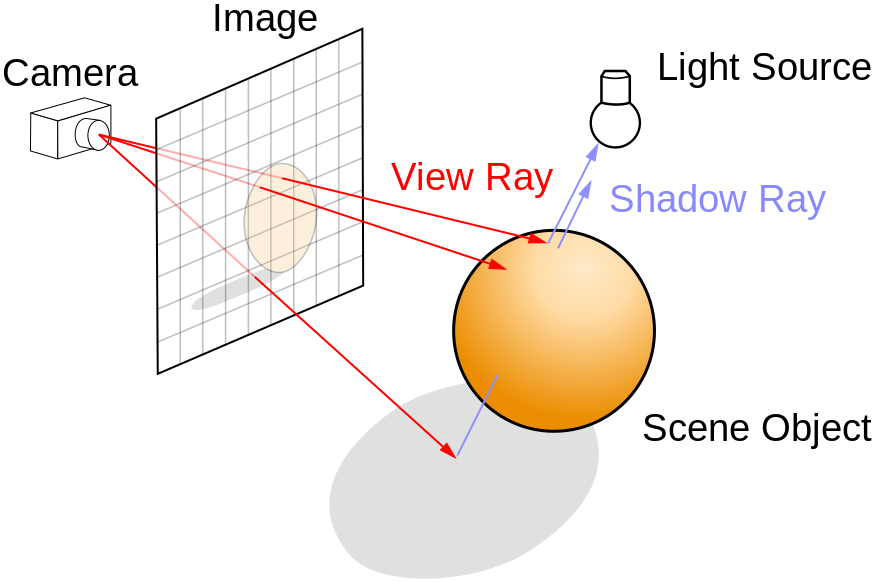
\includegraphics[scale=0.35]{media/Ray_trace_diagram.png}
	\caption{\textit{Ray Casting} algorithm overview. Source: Ray tracing (graphics), Wikipedia}
	\label{globalil}
\end{figure}

Ray tracing uses this mechanism to recursively accumulate the light contribution from reflective and refractive objects. Materials like mirrors or polished metals produce a reflection ray, and transparent or glass objects may produce both reflection and refractive rays. This process occurs recursively, which each new ray may generate new both reflective and refractive rays. Recursion has some cutoff limit, such as a maximum number of bounces (depth). Moreover, the recursion ends when the ray hits a light source or leaves the scene. The number of bounces affects directly to the resultant image. In Figure \ref{bounces}, we can see how the more bounces, the more reflections appear in the rendered image.

\begin{figure}[H]
	\centering
	\medskip
	\begin{subfigure}{.48\textwidth}
		\centering
		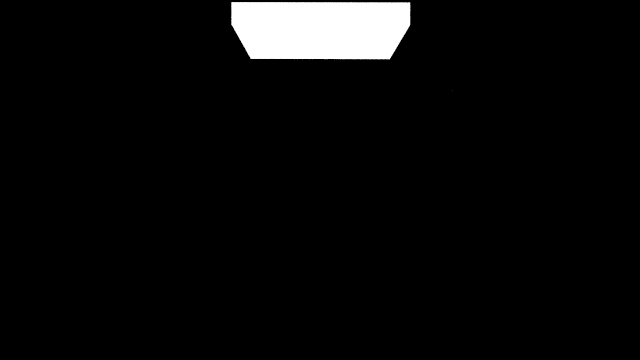
\includegraphics[scale=0.315]{media/mirrors_rect/cornell_mirrors_1.png}
		\caption{1 bounce per ray}
		\label{mr_rect_1}
	\end{subfigure}
	\begin{subfigure}{.48\textwidth}
		\centering
		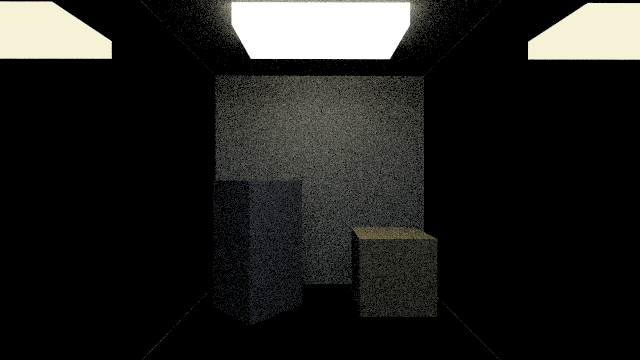
\includegraphics[scale=0.315]{media/mirrors_rect/cornell_mirrors_2.png}
		\caption{2 bounce per ray}
		\label{mr_rect_2}
	\end{subfigure}
	
	\medskip
	\begin{subfigure}{.48\textwidth}
		\centering
		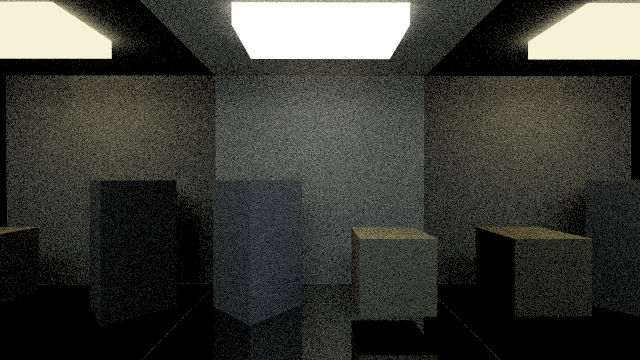
\includegraphics[scale=0.315]{media/mirrors_rect/cornell_mirrors_3.png}	
		\caption{3 bounce per ray}
		\label{mr_rect_3}
	\end{subfigure}		
	\begin{subfigure}{.48\textwidth}
		\centering
		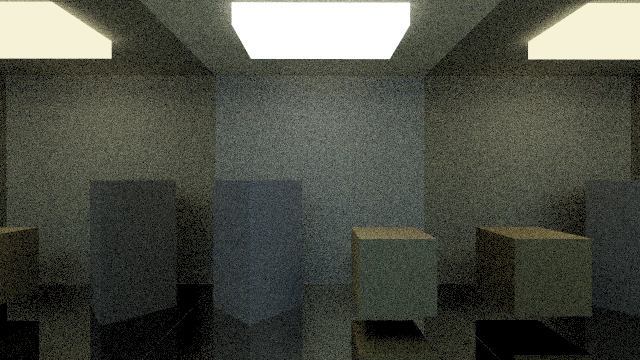
\includegraphics[scale=0.315]{media/mirrors_rect/cornell_mirrors_4.png}
		\caption{4 bounce per ray}
		\label{mr_rect_4}
	\end{subfigure}
	
	\medskip	
	\begin{subfigure}{.48\textwidth}
		\centering
		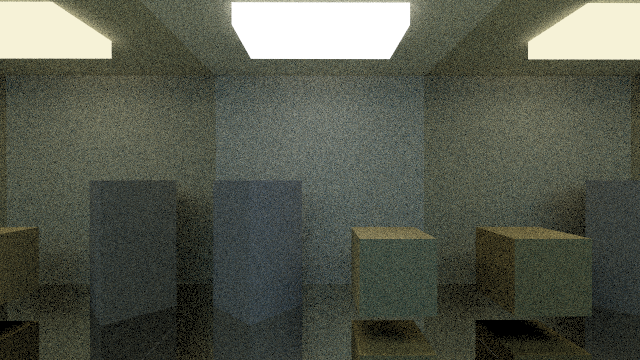
\includegraphics[scale=0.315]{media/mirrors_rect/cornell_mirrors_5.png}
		\caption{5 bounce per ray}
		\label{mr_rect_5}
	\end{subfigure}
	\begin{subfigure}{.48\textwidth}
		\centering
		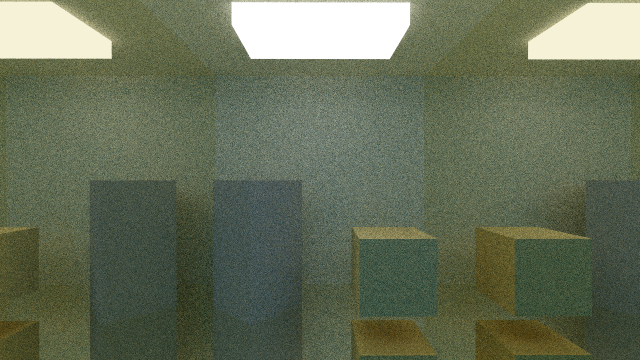
\includegraphics[scale=0.315]{media/mirrors_rect/cornell_mirrors_20.png}	
		\caption{20 bounce per ray}
		\label{mr_rect_20}
	\end{subfigure}
	\caption{Reflections increase with the numbers of bounces.}
	\label{bounces}
\end{figure}


\section{What is a ray?}

\section{Triangles}

\subsection{Materials}

\section{Textures}

\section{BVH}

\newpage

\printbibliography

\begin{appendices}
\chapter{Gantt Diagram}

\uselandscape

\begin{figure}[H]
	\centering
	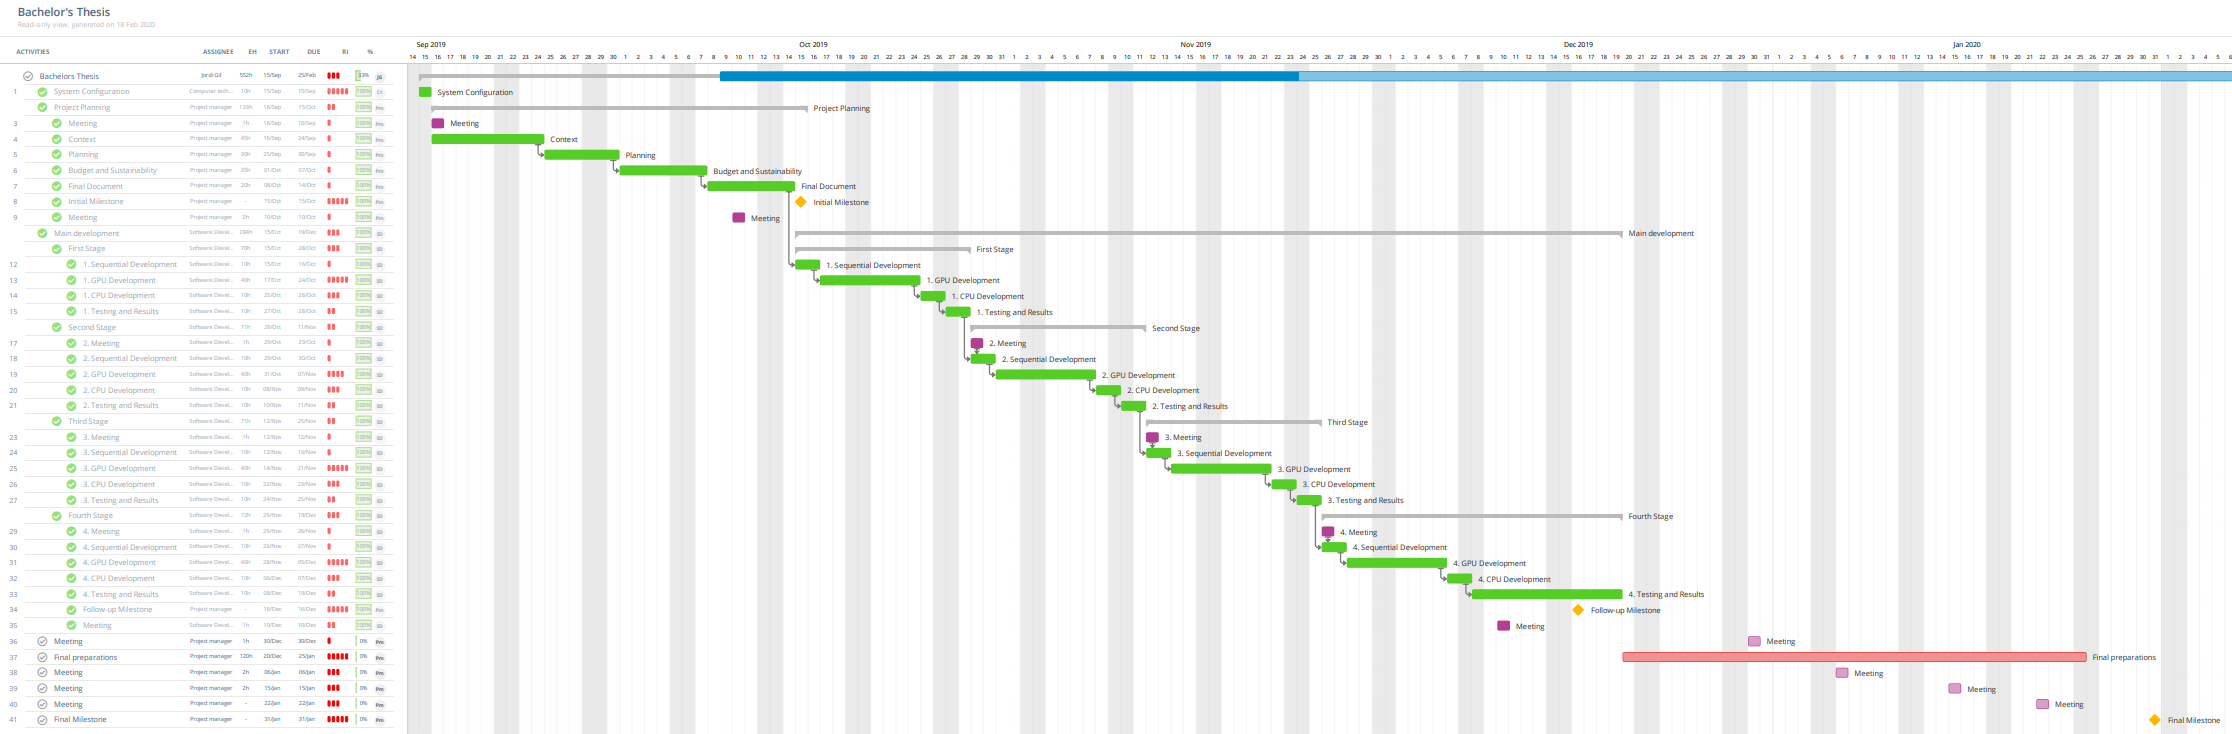
\includegraphics[scale=0.30]{media/final_gantt_esp.png}
	\captionof{figure}{Complete Gantt Chart.}
	\label{gantt_esp}
\end{figure}

\begin{figure}[H]
	\centering
  	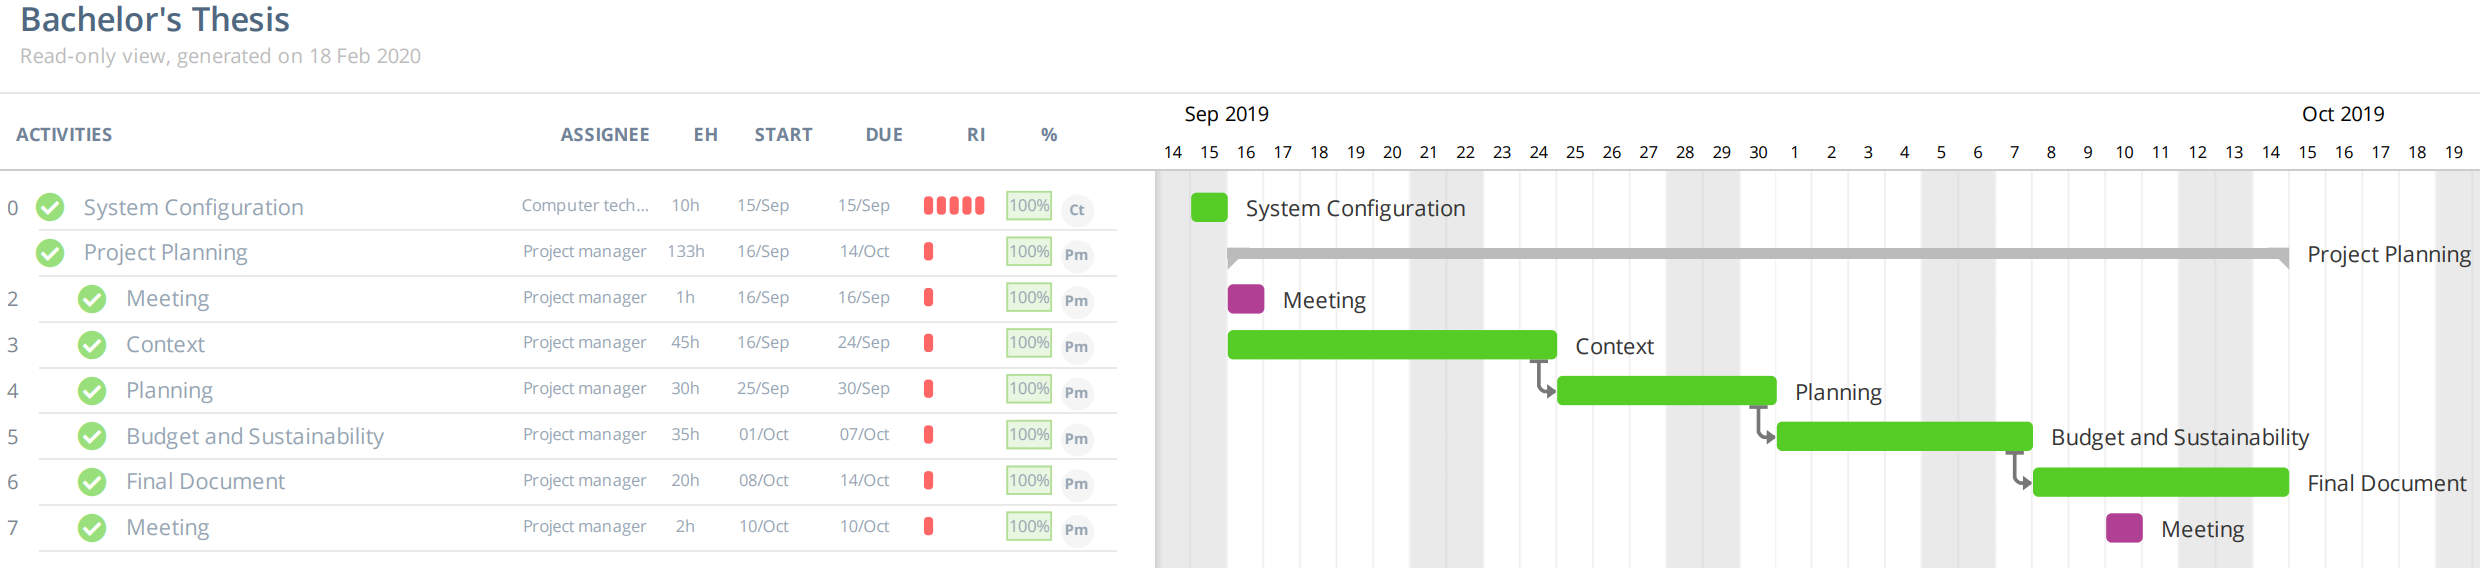
\includegraphics[scale=0.25]{media/gantt_gep.png}
  	\captionof{figure}{GEP Stage.}
  	\label{gantt_1}
\end{figure}

\begin{figure}[H]
	\centering
  	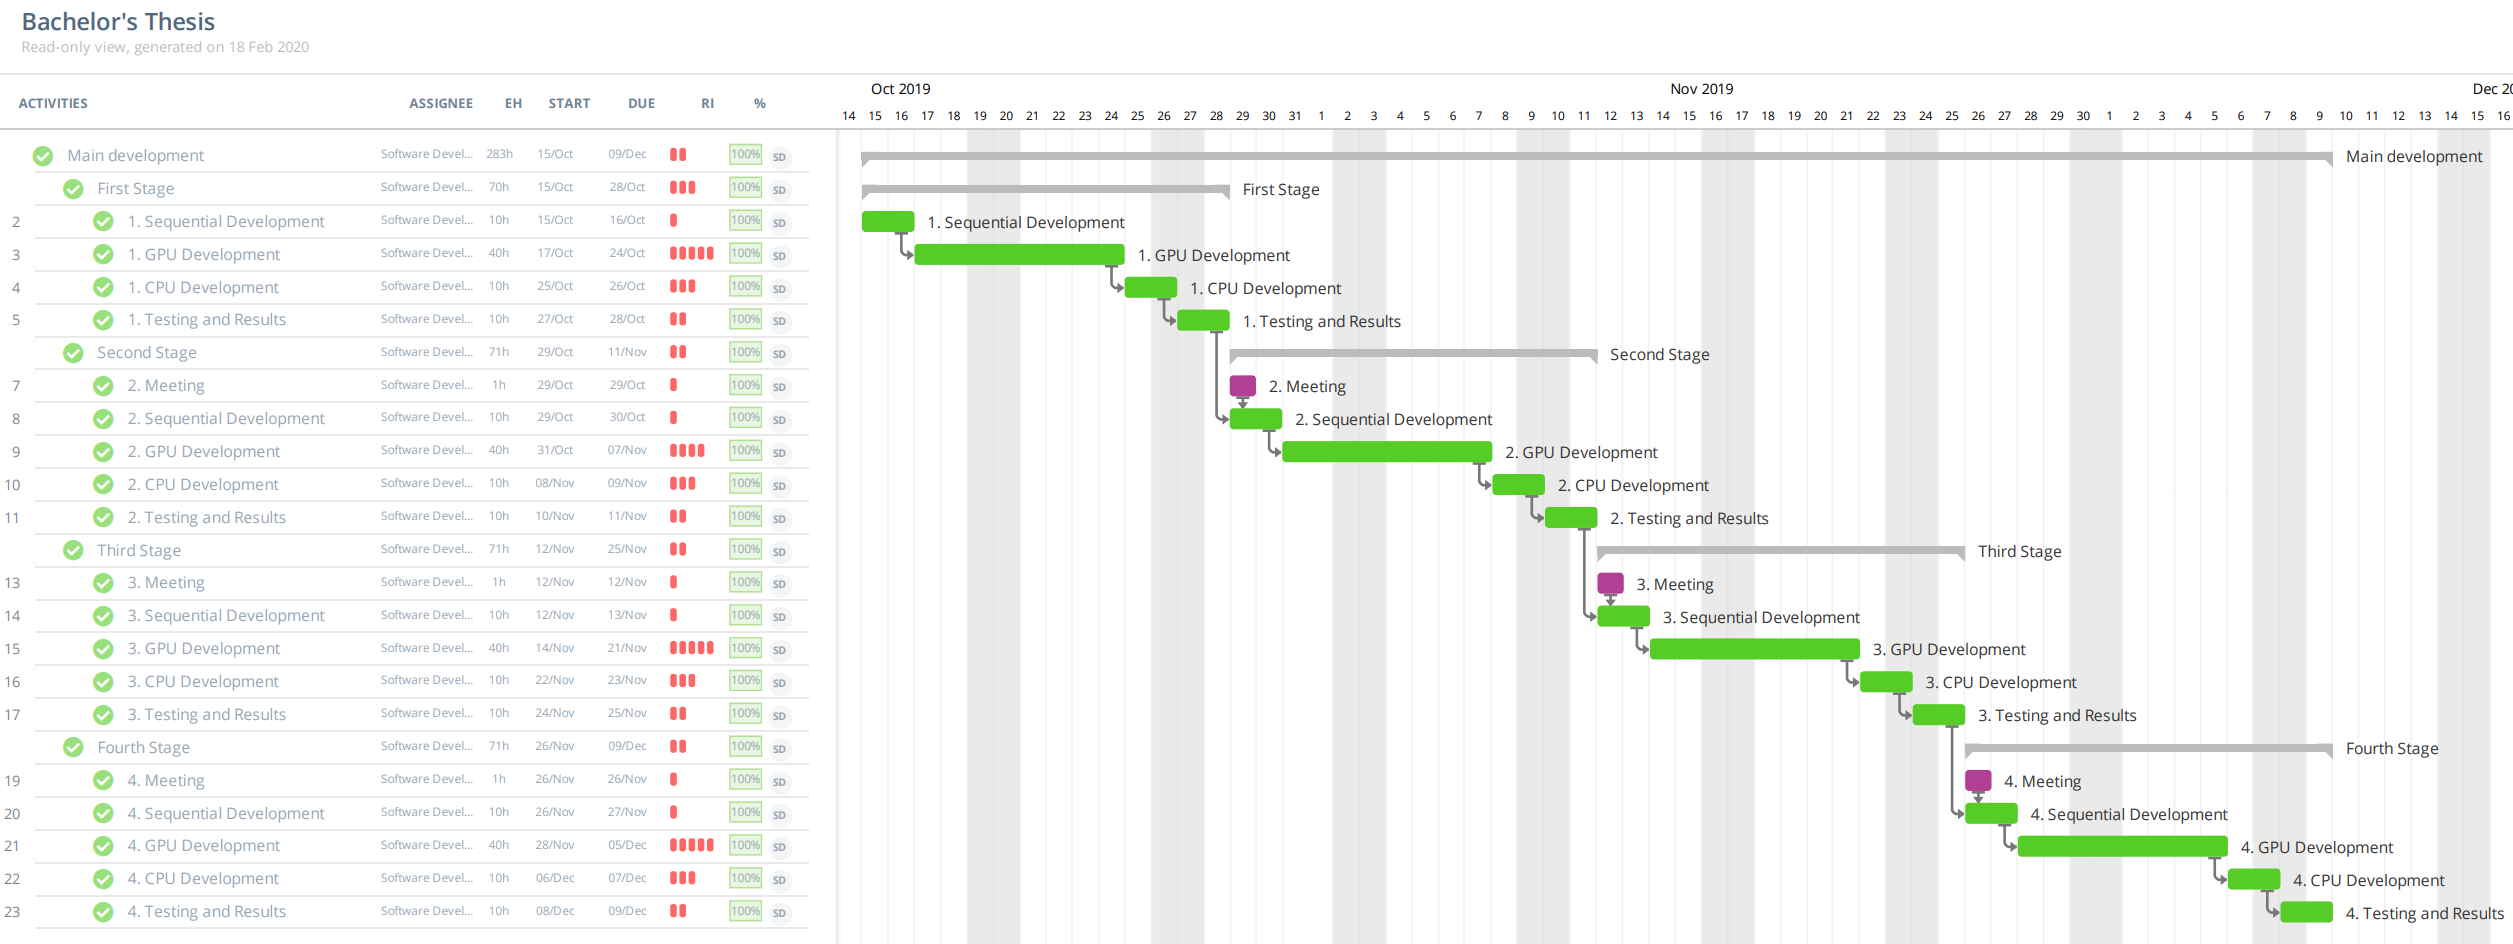
\includegraphics[scale=0.25]{media/gantt_dev_esp.png}
  	\captionof{figure}{Development Stage.}
  	\label{gantt_2}
\end{figure}

\begin{figure}[H]
	\centering
	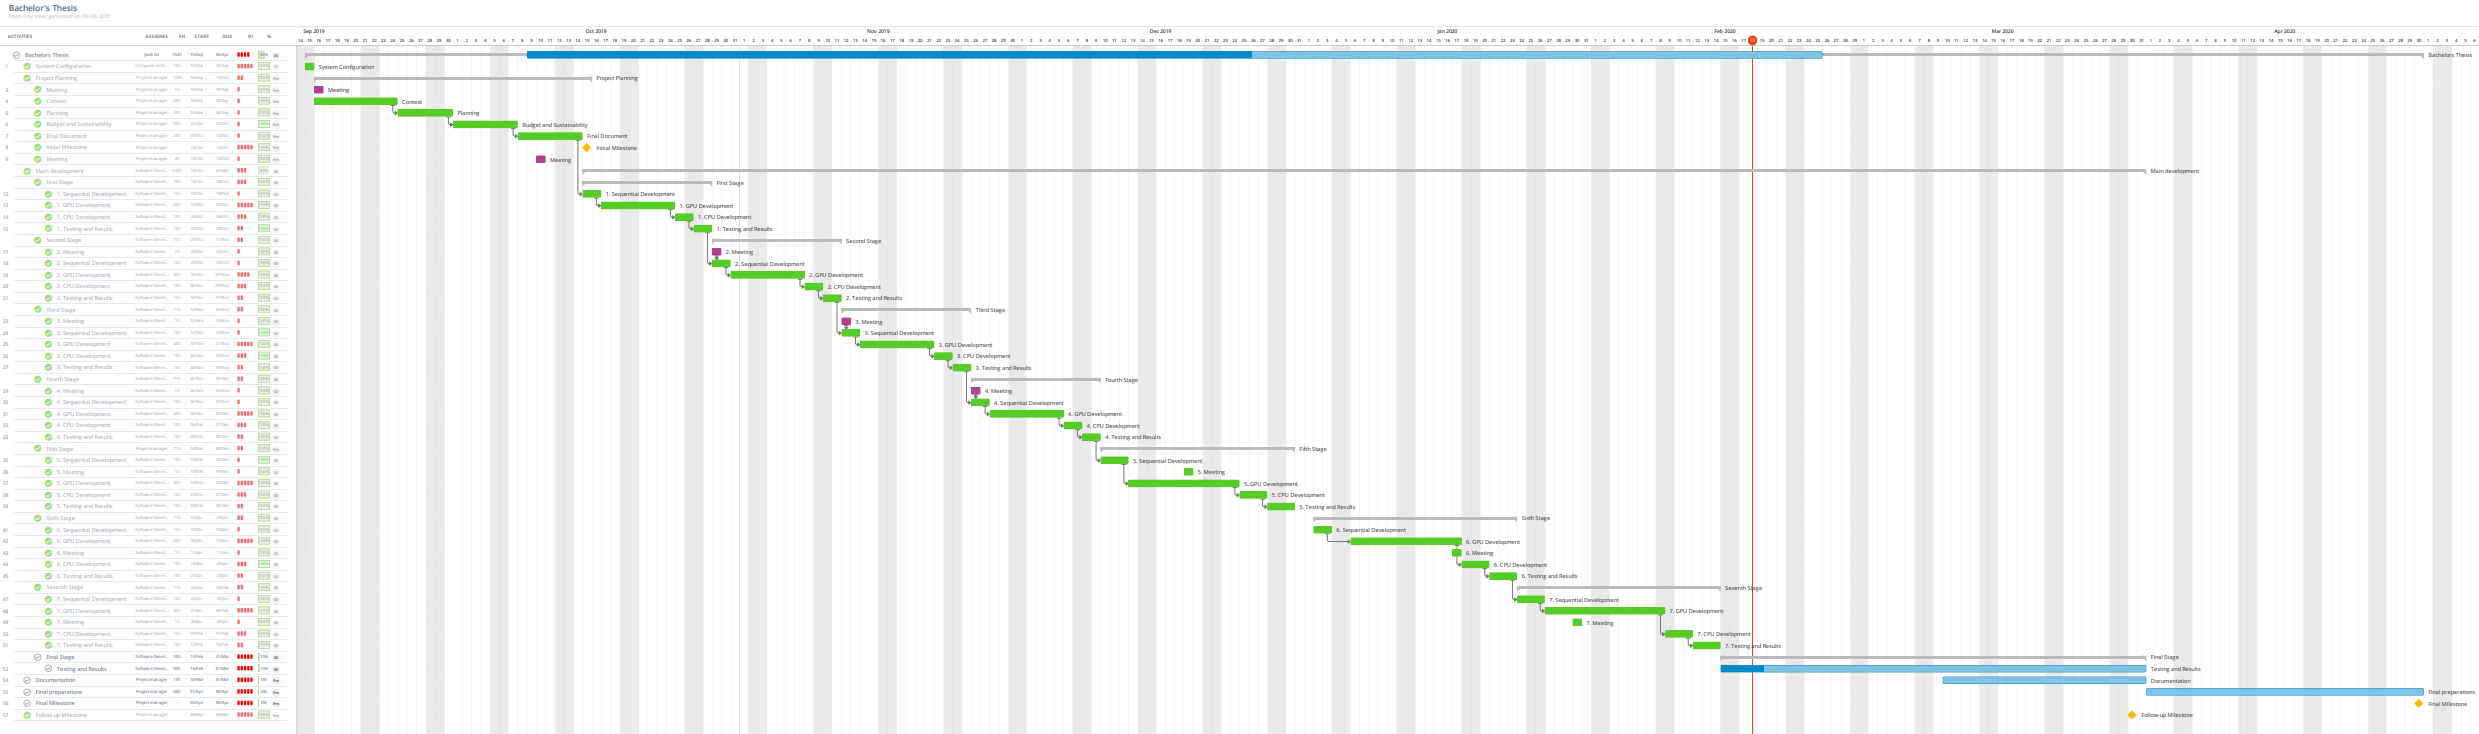
\includegraphics[scale=0.30]{media/final_gantt_eng.png}
	\captionof{figure}{Complete Gantt Chart.}
	\label{gantt_eng}
\end{figure}

\begin{figure}[H]
	\centering
  	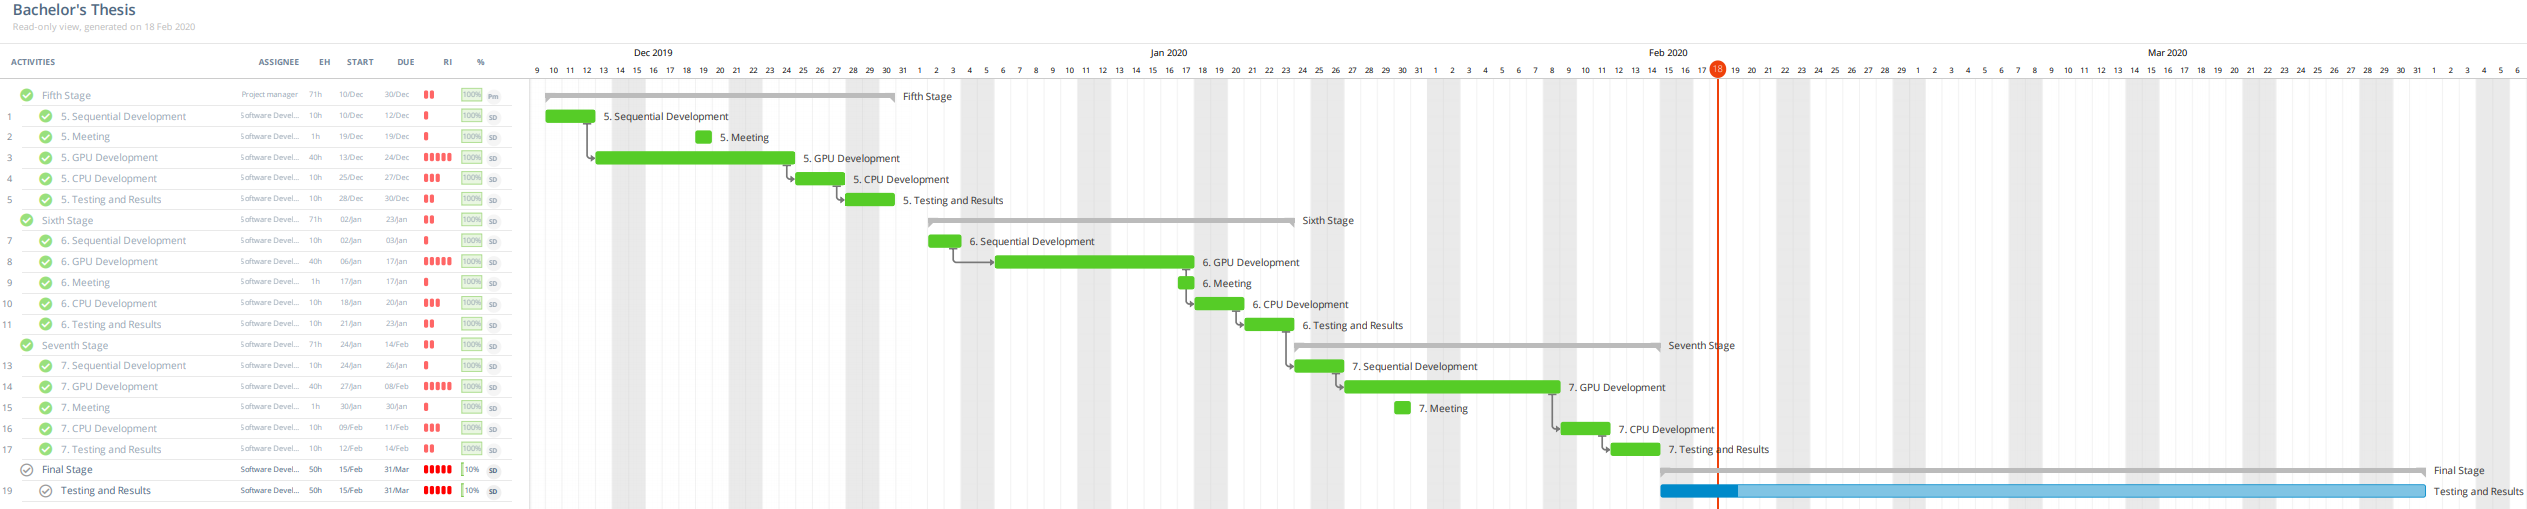
\includegraphics[scale=0.25]{media/gantt_dev_eng_new.png}
  	\captionof{figure}{Development Stage new tasks.}
  	\label{gantt_3}
\end{figure}

\begin{figure}[H]
	\centering
  	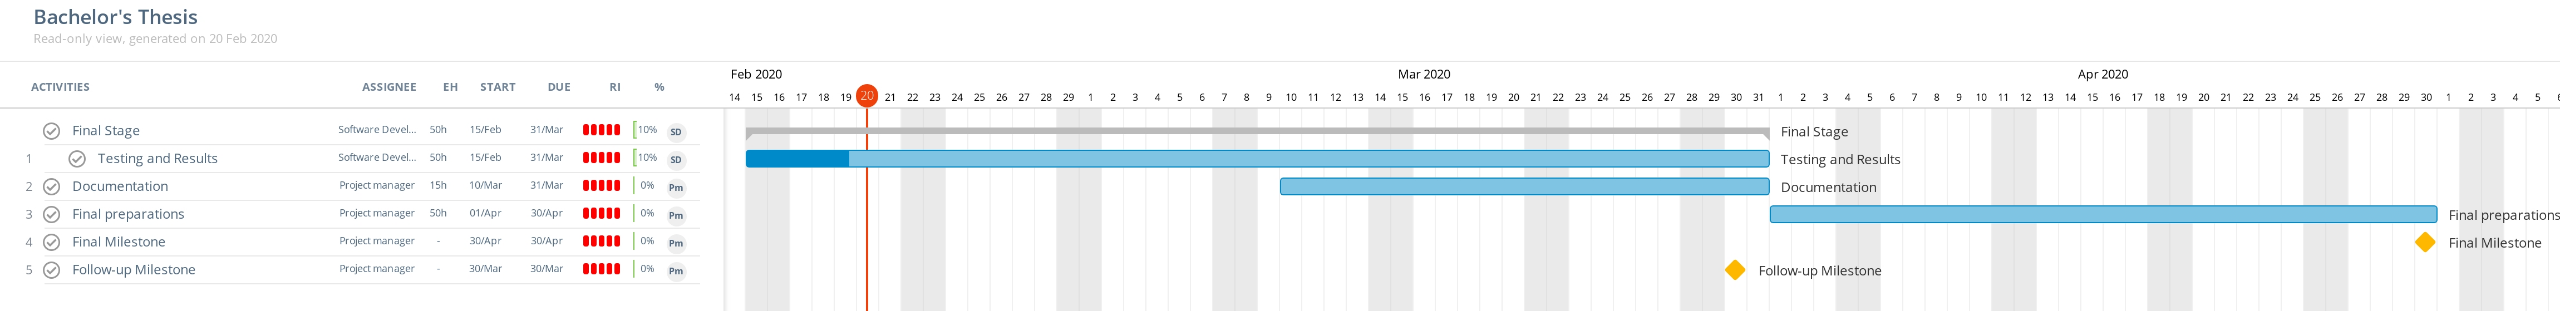
\includegraphics[scale=0.25]{media/gantt_final_eng.png}
  	\captionof{figure}{Final Stage.}
  	\label{gantt_4}
\end{figure}

\useportrait

\end{appendices}

\listoffigures

\listoftables

\end{document}
